\usetikzlibrary{calc}
\usetikzlibrary{arrows.meta}
\usetikzlibrary{positioning}
\usetikzlibrary{shapes.geometric}
\usetikzlibrary{shapes.misc}

\tikzstyle{model} = [rectangle, rounded corners, minimum width=2cm, minimum height=1cm,text centered, draw=black, fill=blue!30]
\tikzstyle{prompt} = [rectangle, rounded corners, minimum width=2cm, minimum height=1cm,text centered, draw=black, fill=red!30]
\tikzstyle{image} = [rectangle, rounded corners, minimum width=2cm, minimum height=1cm, text centered, draw=black, fill=yellow!30]
\tikzstyle{check} = [diamond, minimum height=0.5cm, text centered, draw=black, aspect=3]

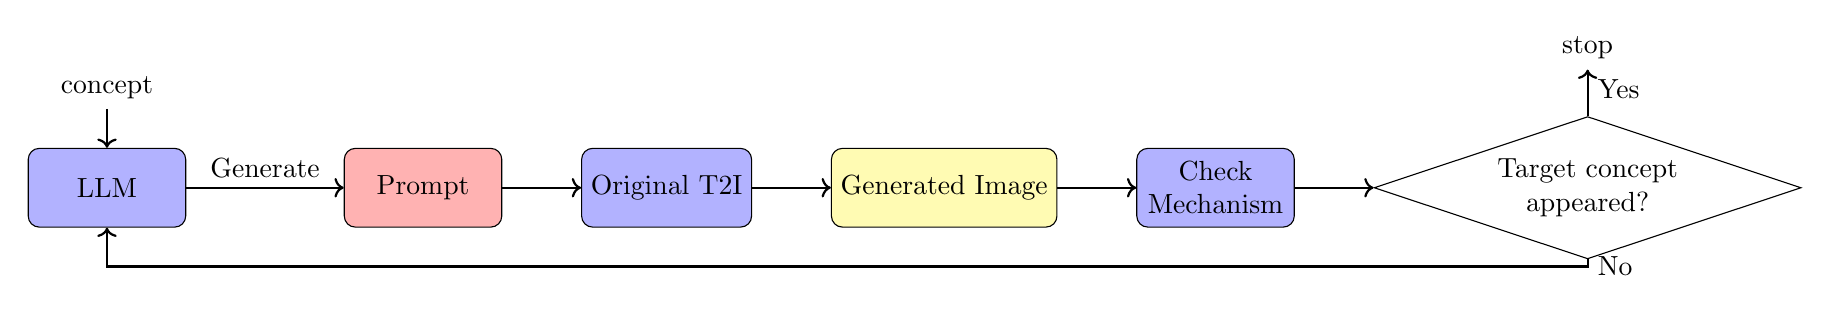
\begin{tikzpicture}[node distance=1cm]
\node[model] (start) {LLM};
\draw[thick, ->] (0, 1) node[above] {concept} -- (start.north);
\node[right=2cm of start, prompt, align=center] (prompt) {Prompt};
\draw[thick, ->] (start) -- (prompt) node[above, pos=0.5] {Generate};
\node[right=of prompt, model] (t2i) {Original T2I};
\draw[thick, ->] (prompt) -- (t2i);

\node[right=of t2i, image, align=center] (output) {Generated Image};
\node[right=of output, model, align=center] (classify) {Check \\ Mechanism};
\draw[thick, ->] (t2i) -- (output);
\draw[thick, ->] (output) -- (classify);

\node[right=of classify, check, align=center] (check) {Target concept \\ appeared?};
\draw[thick, ->] (classify) -- (check);

\draw[thick, ->] (check) -- +(0, -1) node[right] {No} -| (start) node[left, yshift=-15pt] {};
\draw[thick, ->] (check) -- +(0, 1.5cm) node[above] {stop} node[below right] {Yes};
\end{tikzpicture}
